
\begin{frame}{Objectifs du jour}
\begin{itemize}
  \item Mesures de base en classification en TAL : précision, rappel, F-mesure (F$_1$, F$_\beta$)
	  \pause
  \item Mesures de base en RI/ordonnancement : Précision@k, Rappel@k, AP, MAP, DCG / \textbf{nDCG}
	  \pause
  \item Comprendre l'intérêt \textbf{Montrer les limites} de chaque métrique
  \item Lien : du binaire (instance-level) au graduel et ordonné (ranking)
\end{itemize}
\end{frame}

\section{Mesures traditionnelles en TAL/classification}

\begin{frame}{Matrice de confusion (binaire)}
\begin{center}
\begin{tabular}{lcc}
\toprule
 & Prédit + & Prédit - \\
\midrule
Réel + & VP & FN \\
Réel - & FP & VN \\
\bottomrule
\end{tabular}
\end{center}

\vspace{0.6em}
$P=\frac{VP}{VP+FP}$, \quad $R=\frac{VP}{VP+FN}$, \quad $F_1=2\frac{PR}{P+R}$.
\end{frame}

\begin{frame}{Limites (NLP)}
\begin{itemize}
  \item \textbf{Accuracy} trompeuse sur classes déséquilibrées (F1 préférable).
  \item \textbf{Seuil} $\Rightarrow$ compromis précision/rappel (même F1, profils d'erreurs différents).
	  \pause
  \item F1 ignore les \textbf{VN} et le \textbf{coût} asymétrique des erreurs (parfois préférer F$_\beta$).
	  \pause
  \item \textbf{Macro} vs \textbf{Micro} : interprétations différentes.
\end{itemize}
\end{frame}

\section{Mesures en Recherche d'Information (RI)}

\begin{frame}{Spécificités de la RI}
Sortie = \textbf{classement} + \textbf{pertinence} (binaire ou graduelle). Position $\Rightarrow$ utilité.
\end{frame}

\begin{frame}{Mesures principales}
\begin{itemize}
  \item \textbf{P@k}, \textbf{R@k} : qualité sur le top-$k$
  \item \textbf{AP} (binaire) et \textbf{MAP} (moyenne multi-requêtes)
  \item \textbf{DCG}/\textbf{nDCG} : pertinence graduelle + \textit{discount} par rang
\end{itemize}
\end{frame}

\begin{frame}{Limites (RI)}
\begin{itemize}
  \item P@k sensible au \textbf{cutoff} $k$
  \item R@k dépend du \textbf{pool} de pertinents (jugements incomplets)
  \item MAP masque la \textbf{variance} entre requêtes
  \item nDCG sensible au \textbf{gain} (linéaire vs exponentiel) et au \textbf{cutoff}
\end{itemize}
\end{frame}

\section{Passer par le visuel}

\begin{frame}{Courbe PR (classification)}
\begin{figure}
\centering
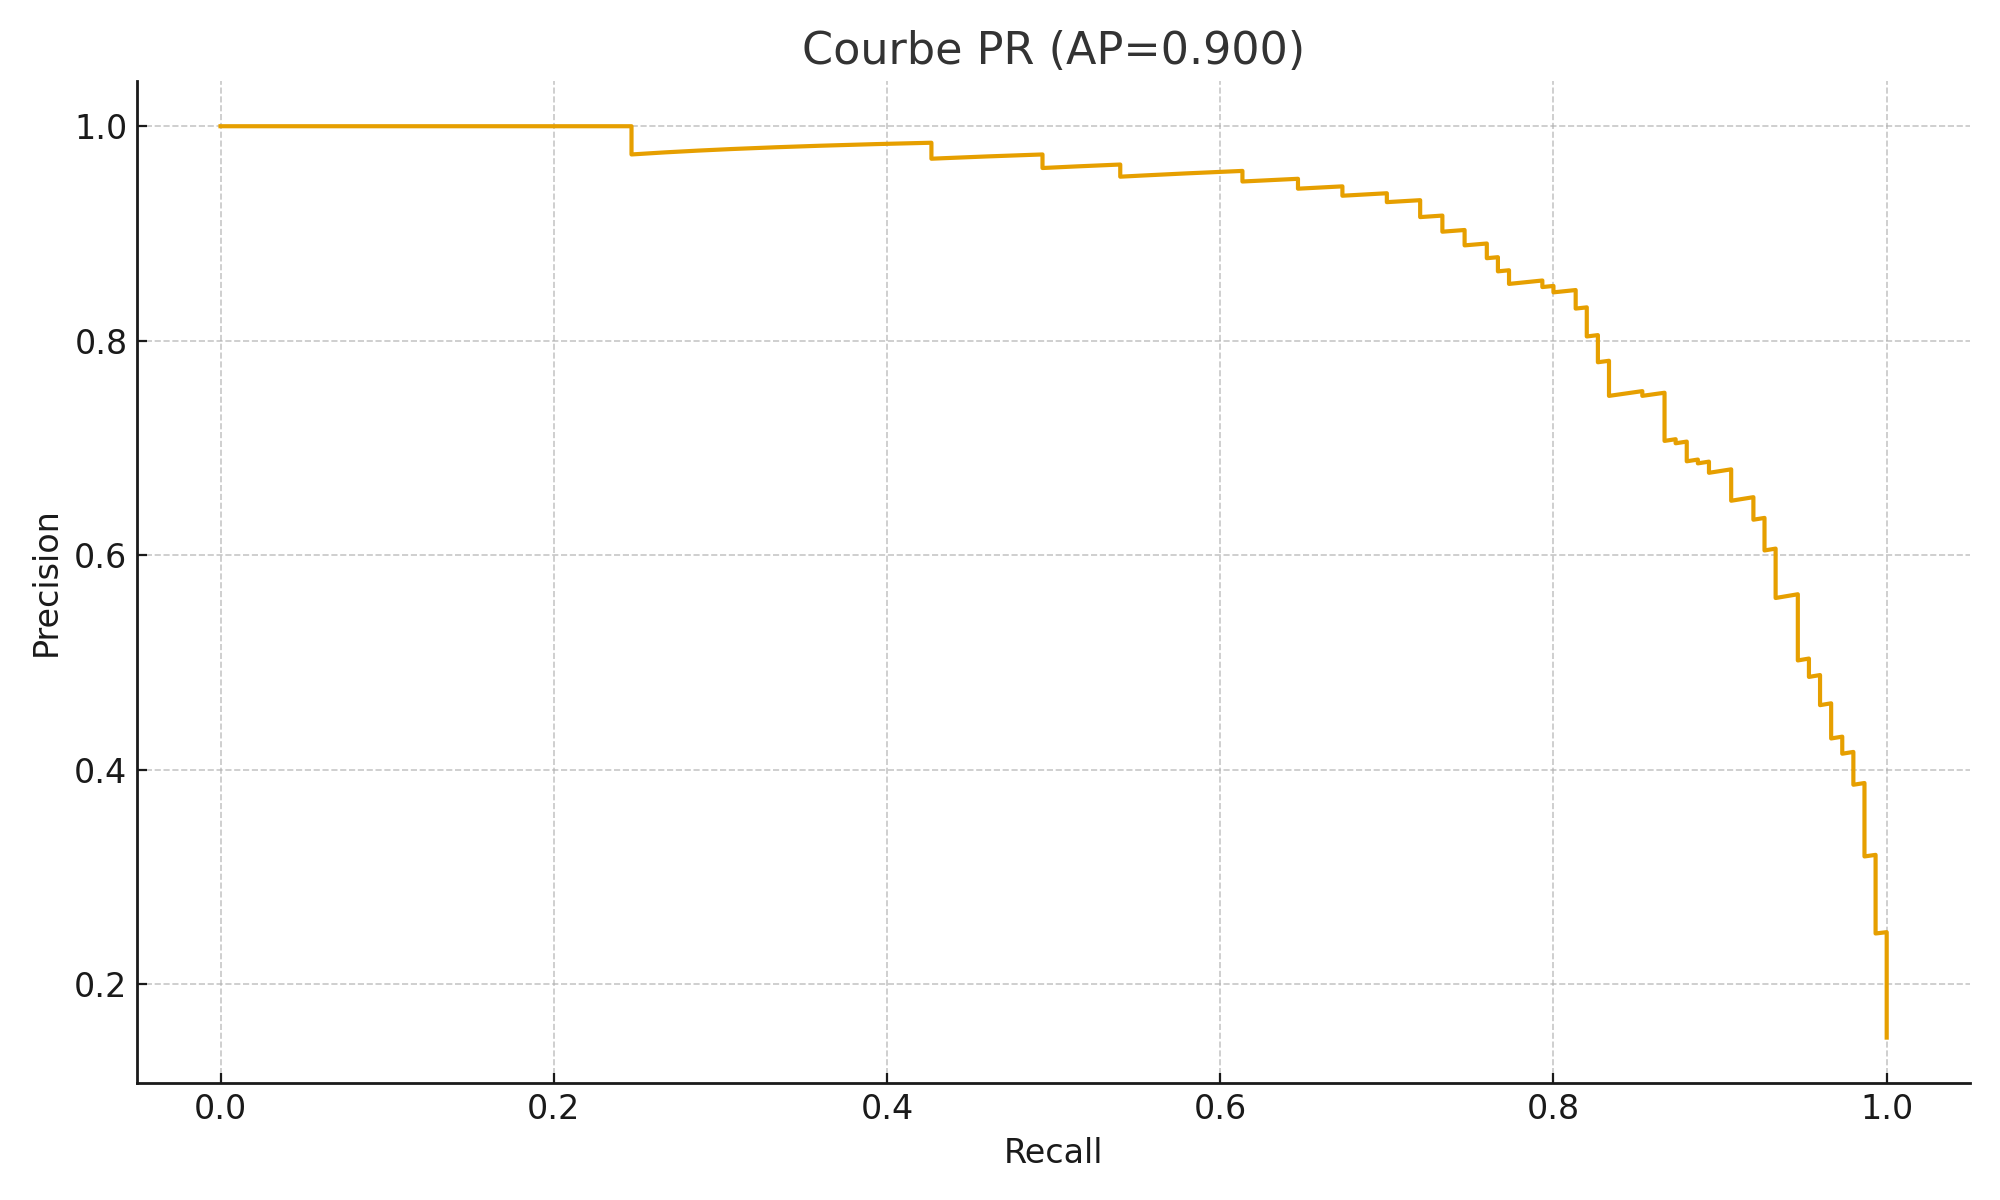
\includegraphics[width=\textwidth]{parts/pr_curve.png}
\end{figure}
\end{frame}

\begin{frame}{Courbe ROC (classification)}
\begin{figure}
\centering
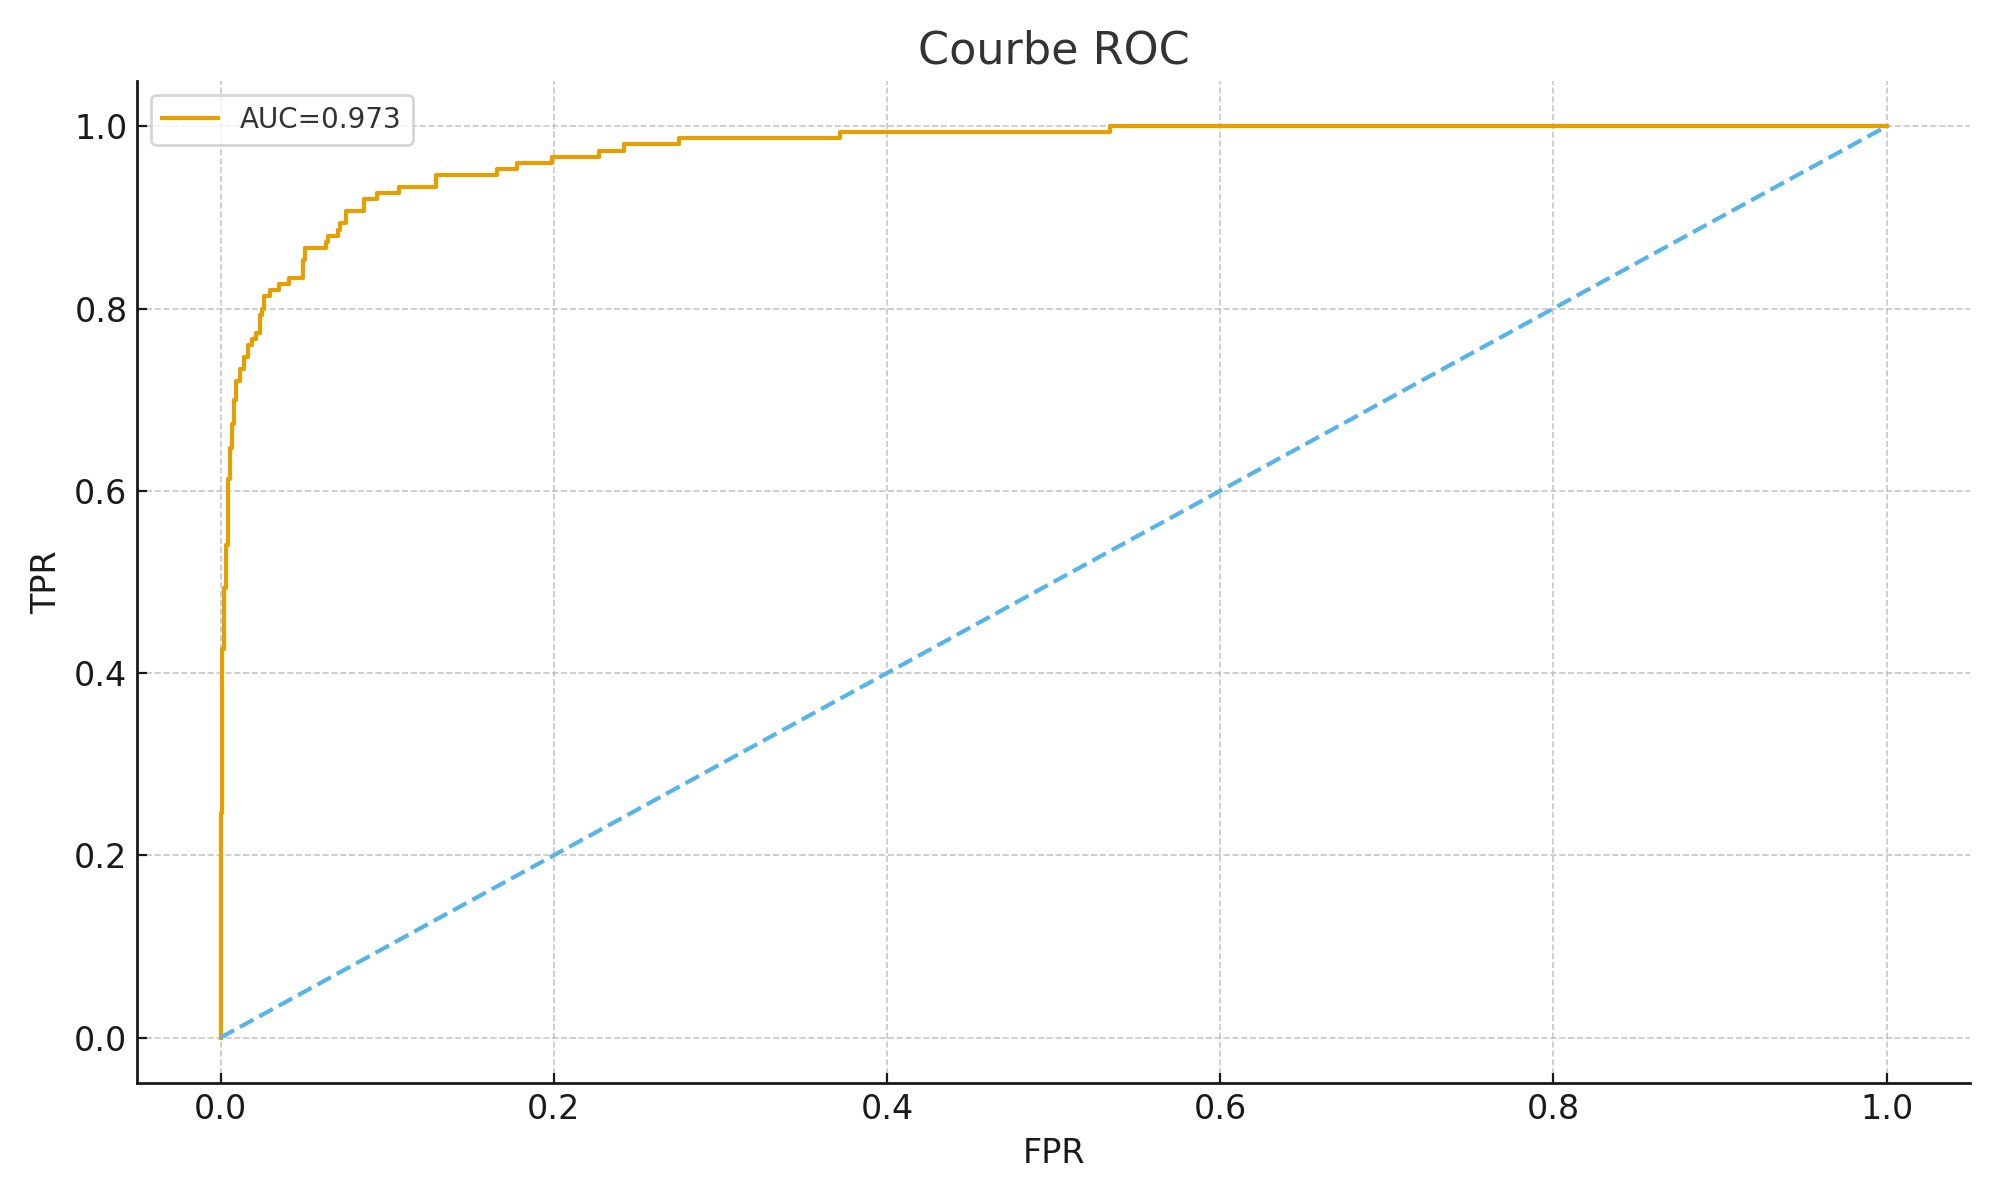
\includegraphics[width=\textwidth]{parts/roc_curve.png}
\end{figure}
\end{frame}

\begin{frame}{Multiclasse : erreurs et déséquilibre}
\begin{figure}
\centering
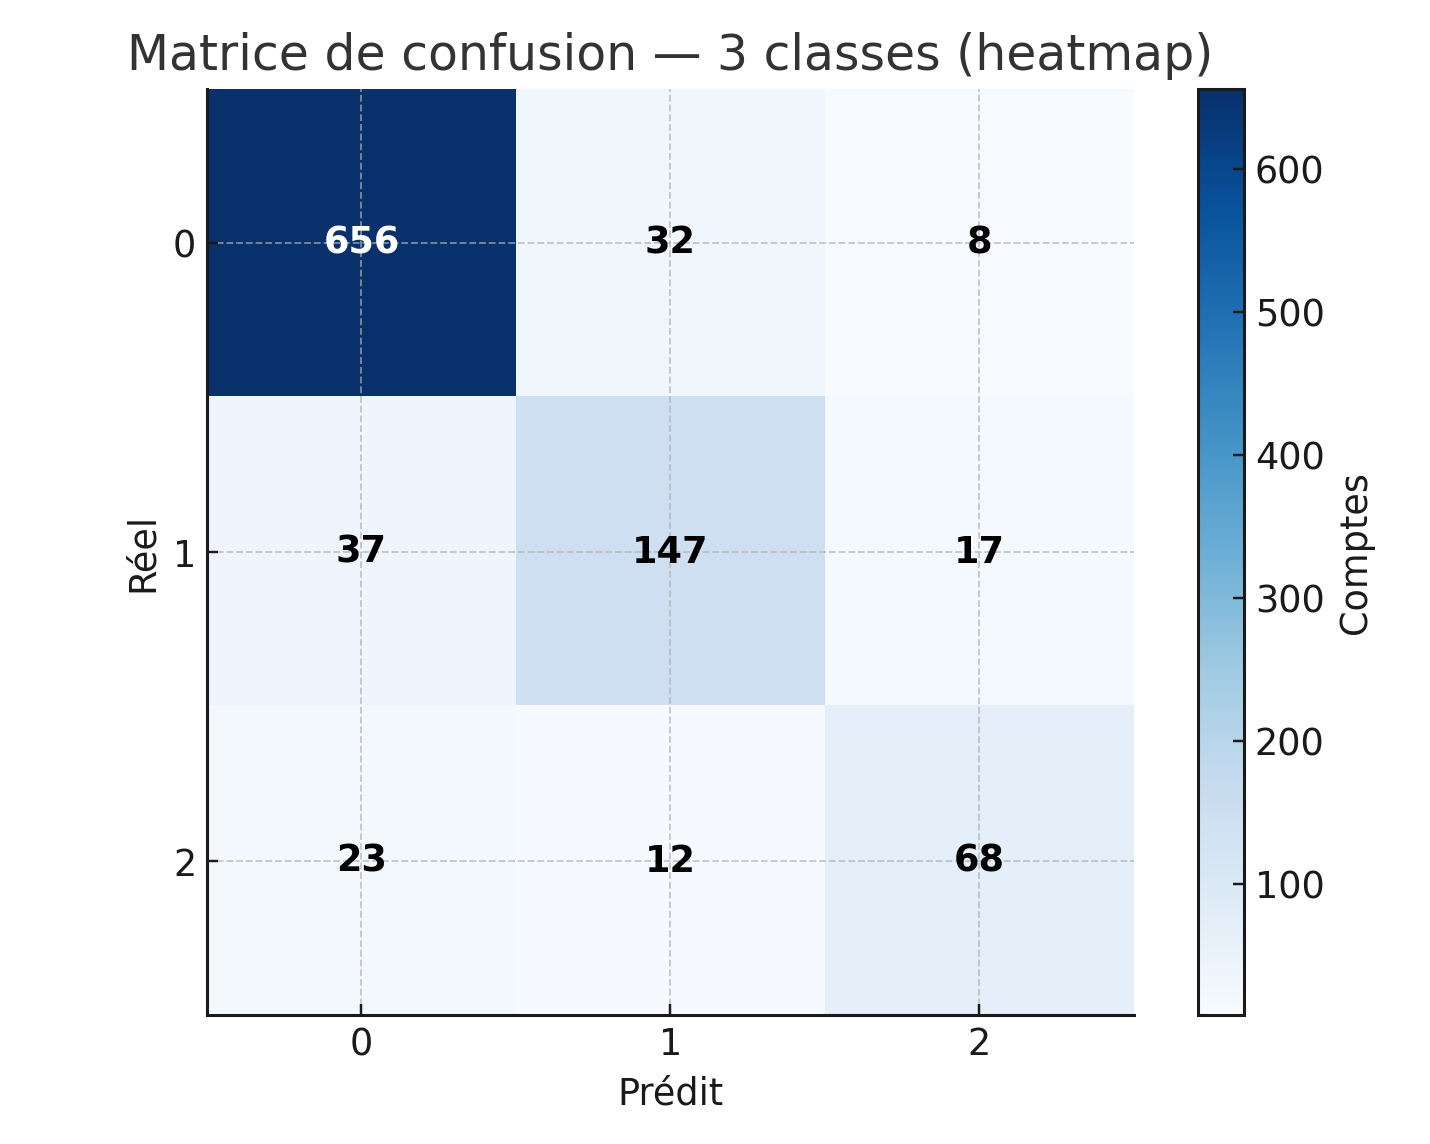
\includegraphics[width=\textwidth]{parts/multiclass_confusion.png}
\end{figure}
\end{frame}

\begin{frame}{nDCG : gain linéaire vs exponentiel}
\begin{figure}
\centering
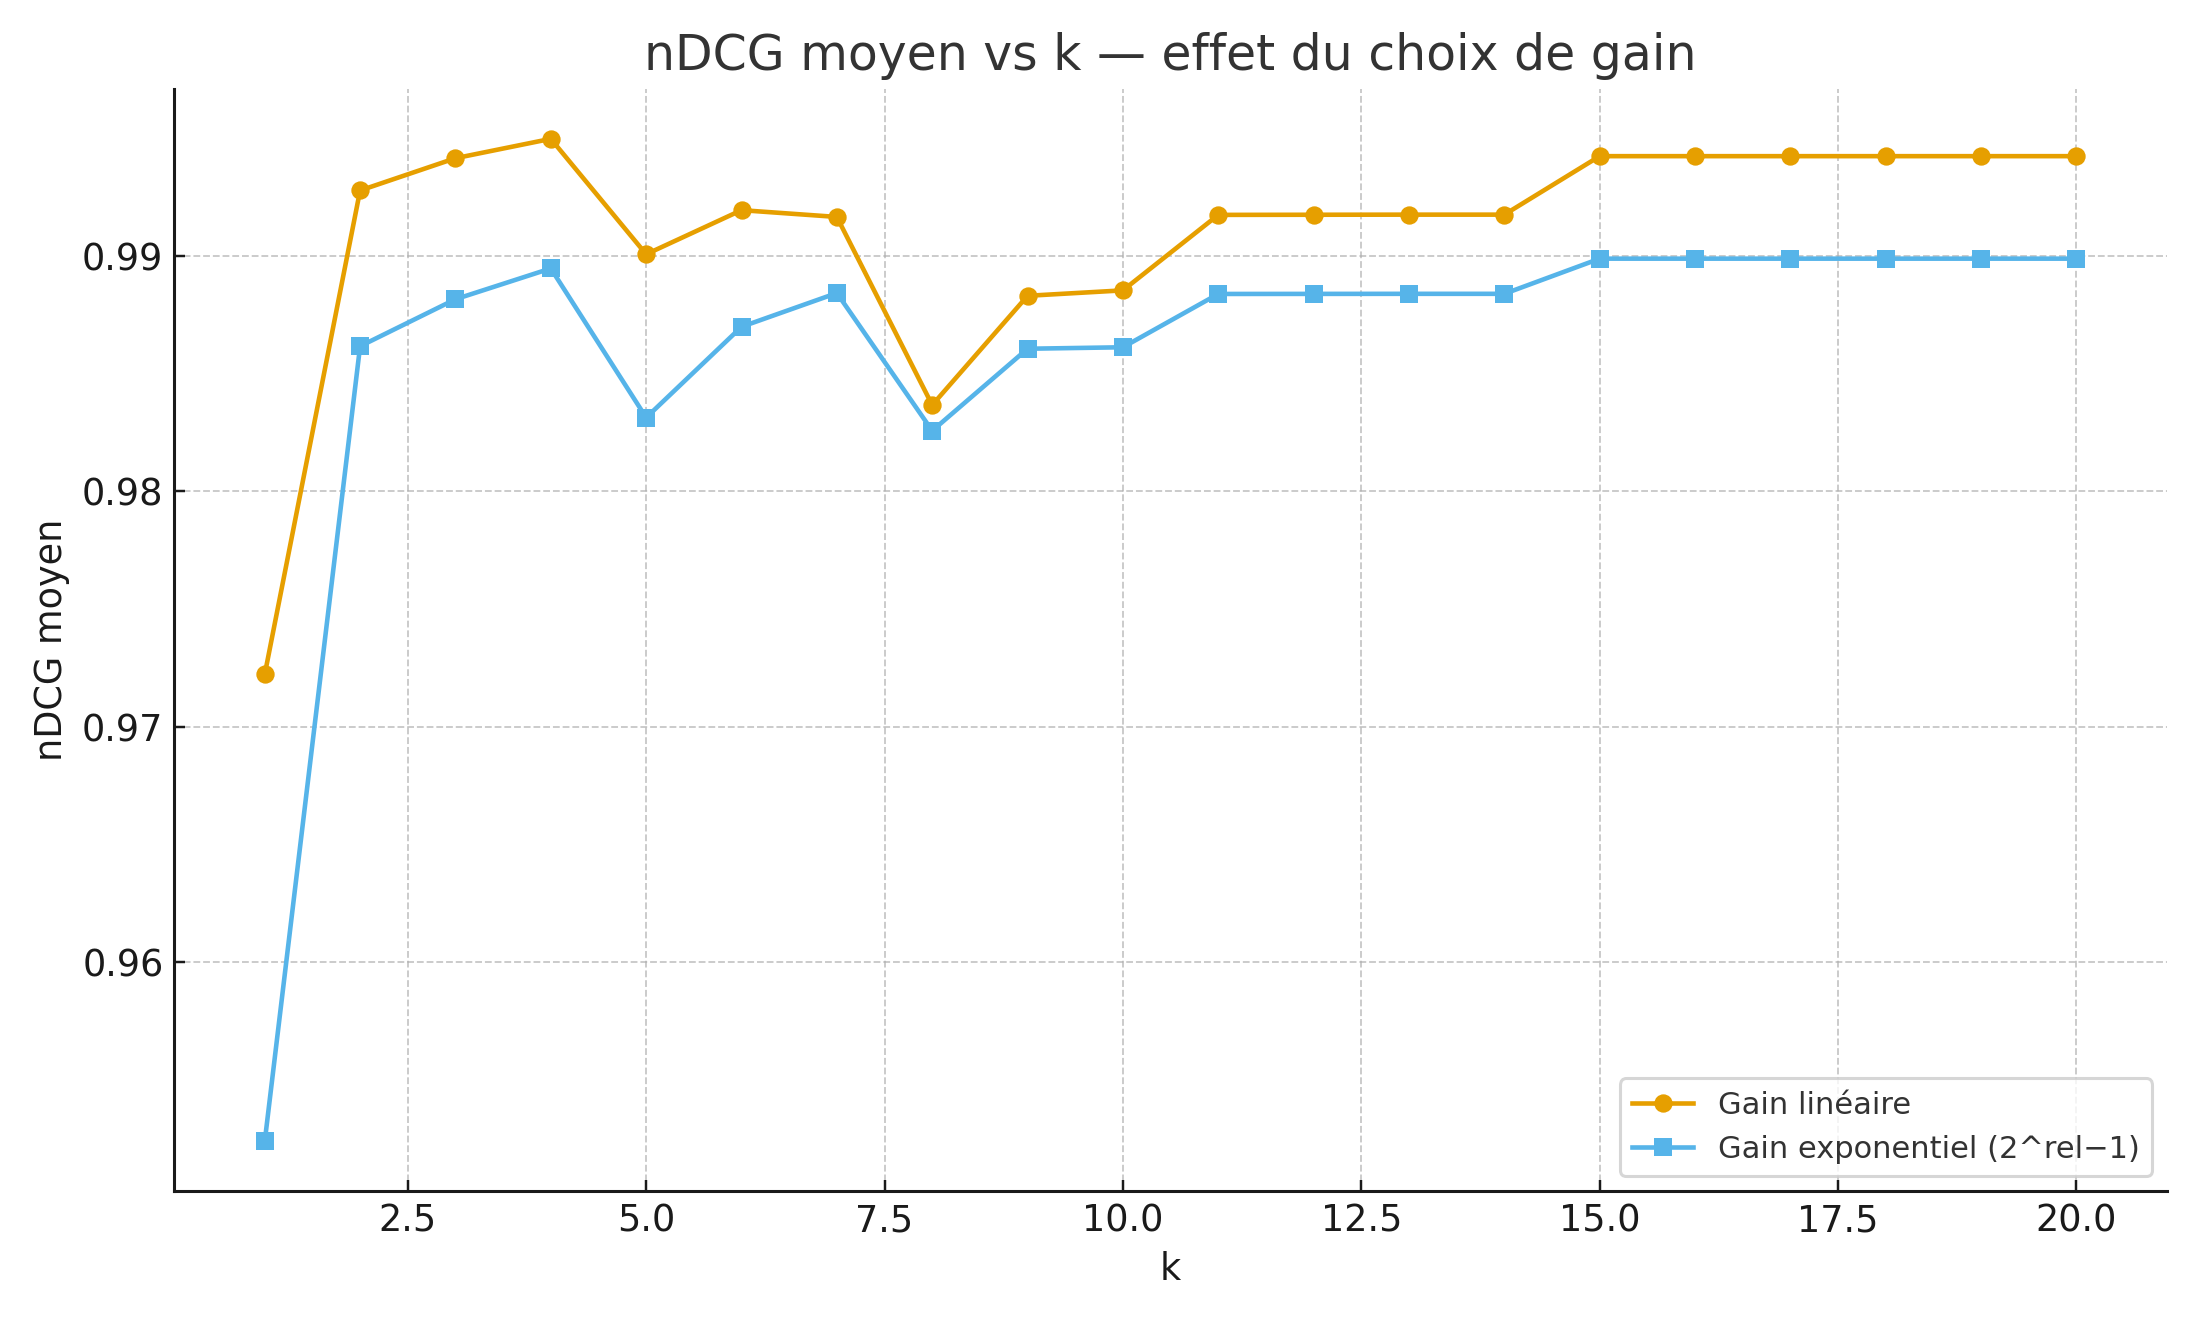
\includegraphics[width=\textwidth]{parts/ndcg_compare.png}
\end{figure}
\end{frame}

\begin{frame}{nDCG — interprétation du gain linéaire vs exponentiel}

%\textbf{Formule générale :}
\[
\text{DCG@k} = \sum_{i=1}^k \frac{g_i}{\log_2(i+1)} \qquad 
\text{où } g_i = \text{gain}(rel_i)
\]

\begin{block}{Deux choix possibles pour la fonction de gain}
\begin{itemize}
    \item \textbf{Gain linéaire} : $g(rel) = rel$  
    $\Rightarrow$ chaque niveau de pertinence ajoute une valeur proportionnelle.
    \item \textbf{Gain exponentiel} : $g(rel) = 2^{rel}-1$  
    $\Rightarrow$ les documents très pertinents comptent beaucoup plus.
\end{itemize}
\end{block}

\begin{center}
\begin{tabular}{ccccc}
\toprule
Niveau de pertinence & 0 & 1 & 2 & 3 \\
\midrule
Gain linéaire & 0 & 1 & 2 & 3 \\
Gain exponentiel & 0 & 1 & 3 & 7 \\
\bottomrule
\end{tabular}
\end{center}
\end{frame}

\begin{frame}{nDCG — interprétation du gain linéaire vs exponentiel}
\begin{center}
\begin{tabular}{ccccc}
\toprule
Niveau de pertinence & 0 & 1 & 2 & 3 \\
\midrule
Gain linéaire & 0 & 1 & 2 & 3 \\
Gain exponentiel & 0 & 1 & 3 & 7 \\
\bottomrule
\end{tabular}
\end{center}
\vspace{0.5em}
\textbf{Interprétation :}
\begin{itemize}
  \item Le \textbf{gain linéaire} favorise la régularité : plusieurs résultats pertinents suffisent.
  \item Le \textbf{gain exponentiel} surpondère les très pertinents : utile pour les classements courts (web search).
\end{itemize}

\end{frame}


\section{Synthèse}

\begin{frame}{Quel indicateur pour quel usage ?}
\begin{itemize}
  \item \textbf{Filtrage strict} : précision élevée (F$_\beta$, $\beta<1$), PR-curve.
	  \pause
  \item \textbf{Veille signaux faibles} : rappel prioritaire (F$_\beta$, $\beta>1$), AP (classification).
	  \pause
  \item \textbf{Recherche Info} : P@k, nDCG@k (petits $k$), Mean Average Precision.
%  \item \textbf{Reporting} : plusieurs $k$, macro/micro, distribution des AP, seeds/splits.
\end{itemize}
\end{frame}

